\documentclass[runningheads]{llncs}

\usepackage[T1]{fontenc}
\usepackage[utf8]{inputenc}
\usepackage{graphicx}
\usepackage{booktabs}
\usepackage{amsmath}
\usepackage{amssymb}
\usepackage{siunitx}
\usepackage{multirow}
\usepackage{url}
\usepackage{xcolor}
\usepackage{placeins}
\graphicspath{{./figuras/}}

\title{Water Quality Prediction: Energy-Aware Offline Multimodal Neuromorphic Edge Inference}
\titlerunning{Energy-Aware Offline Neuromorphic Edge Inference}

\author{
Felipe de Vasconcelos Assunção\inst{1} \and
Alfredo Paulo Oliveira Barros\inst{1} \and
Reyner Carlos Silva Alegria\inst{1} \and
Elton dos Santos Araújo\inst{2} \and
Débora Romano Raimundo\inst{3} \and
Alex Martins Ramos\inst{1} \and
Vicente Ferreira de Lucena Junior\inst{1} \and
Vandermi João da Silva\inst{1}
}

\authorrunning{Assunção et al.}

\institute{
Federal University of Amazonas (UFAM), Institute of Exact and Technological Sciences (ICET), Itacoatiara, Brazil \\
\email{\{felipe.assuncao, alfredo.barros, reyner.alegria, alexmartins, vicente, vandermi\}@ufam.edu.br}
\and
Independent Researcher, Brazil \\
\email{elton\_araujo\_@hotmail.com}
\and
Eldorado Research Institute, Brazil \\
\email{debora.raimundo@eldorado.org.br}
}

\begin{document}
\maketitle

\begin{abstract}
This work investigates energy-aware neuromorphic edge inference for multimodal water quality prediction in a remote Amazonian region of northern Brazil. A spiking neural network (SNN) is deployed on low-cost embedded platforms to jointly predict pH, dissolved oxygen, and turbidity directly from georeferenced physicochemical measurements, without reliance on cloud connectivity. To mitigate the limited size of the field dataset, light Gaussian augmentation is employed to improve training stability. The SNN architecture, based on a leaky integrate-and-fire hidden layer, is optimized through systematic grid search over temporal steps, learning rate, threshold, decay factor, and hidden-layer size. The final model achieves competitive predictive performance while enabling fully offline inference on constrained hardware. Latency and energy benchmarks are reported across Raspberry Pi, Android devices, and ESP32 platforms, including INA219-based power telemetry and incremental energy-per-inference estimates derived from idle and load measurements. Results demonstrate the feasibility of neuromorphic inference for autonomous environmental monitoring, revealing measurable energy-latency trade-offs and supporting deployment in connectivity- and power-limited scenarios.

\keywords{Spiking Neural Networks \and Edge AI \and Energy Benchmarking \and Water Quality Prediction \and Multimodal Modeling \and Offline Inference}
\end{abstract}

\section{Introduction}

Water-quality monitoring in remote Amazonian areas is constrained by sparse infrastructure, high field logistics cost, and intermittent network connectivity. In this context, continuous dependence on cloud inference is operationally fragile and energetically expensive, especially for battery-powered deployments and long-duration campaigns. At the same time, water-quality variables such as pH, dissolved oxygen (OD), and turbidity are highly relevant for environmental screening and public-health risk mitigation.

Conventional machine-learning pipelines can provide strong predictive performance, but many are designed for server-centric execution and do not directly address energy constraints at the edge. Neuromorphic models based on spiking neural networks (SNNs) offer an alternative computational paradigm with event-driven processing and potential compatibility with low-power embedded systems. However, practical evidence in real environmental sensing workflows remains limited, particularly when combining multimodal prediction and platform-level energy benchmarking.

This paper proposes and evaluates an offline multimodal SNN pipeline for water-quality prediction in an Amazonian field scenario, including end-to-end deployment and cross-platform energy analysis. The study integrates data processing, model training, geospatial interpretation, and embedded inference on heterogeneous hardware (ESP32, Raspberry Pi, and Android devices).

The main contributions of this work are an offline multimodal SNN approach for joint prediction of pH, OD, and turbidity from georeferenced physicochemical inputs, a reproducible energy-measurement protocol based on INA219 incremental idle/load estimation across embedded and mobile platforms, a comparative latency--energy analysis that exposes practical trade-offs between microcontroller, SBC, and smartphone execution, and an applied environmental case study in the Amazon region with spatial visualization and operational pollution-index mapping.

\section{Related Work}

\subsection{Water Quality Prediction}
Data-driven prediction of water-quality indicators has been widely explored with ANN, tree-based models, and recurrent architectures. Reviews and recent studies report consistent use of physicochemical variables and geospatial context for forecasting pH, OD, turbidity, and composite indicators \cite{yan2024,ahmed2019,aladhaileh2021}. LSTM-based approaches are common where temporal records are dense \cite{liu2019,pyo2023}, while hybrid and ensemble methods improve robustness under nonlinear behavior and limited sample regimes \cite{wu2022,chadalavada2025}.

Beyond model choice, an important distinction in the literature is the operational objective: some studies prioritize maximum predictive accuracy in centralized infrastructure, while others prioritize robustness under noisy sensing, sparse sampling, and field constraints. For inland-water applications, this distinction is critical because model behavior is affected by local heterogeneity, seasonality, and variable measurement uncertainty. Recent environmental AI surveys report that small-to-medium tabular datasets remain common in practice, which motivates regularization, repeated-seed evaluation, and careful interpretation of metric differences \cite{yan2024,lowe2022}.

Another relevant point is target coupling. Predicting pH, OD, and turbidity independently can improve per-variable tuning, but joint multimodal prediction better reflects field decision workflows in which variables are interpreted together. Multitarget learning therefore offers operational advantages for screening and prioritization, even when one target (typically turbidity) remains harder to model due to stronger local variability and nonlinear effects.

\subsection{Edge AI and Energy Evaluation}
For environmental IoT deployments, inference cost must be evaluated jointly with predictive quality. Prior work highlights the relevance of platform-level benchmarking and hardware-aware model design \cite{rosero2020,zulkifli2022}. Recent neuromorphic and energy-efficient AI studies indicate that event-driven models can be attractive for constrained settings, but deployment evidence across heterogeneous edge hardware is still developing \cite{aral2024,azadi2025,huijbregts2024}. This gap motivates the present work: a unified comparison of offline multimodal inference quality and energy-per-inference behavior on multiple practical platforms.

Most prior studies report either algorithmic metrics or hardware metrics in isolation. In contrast, field deployment requires a coupled view of latency, throughput, and incremental energy under realistic idle/load transitions. This is particularly important on mobile and embedded systems where background services, CPU governors, and interpreter/runtime overhead can substantially change effective energy per inference. Consequently, cross-platform benchmarking should be interpreted as a systems result, not only as a model result.

From the neuromorphic perspective, software-executed SNNs on conventional CPUs may not always minimize absolute energy compared with optimized dense models, but they provide architectural compatibility with event-driven computation and a direct migration path to dedicated neuromorphic hardware. This makes SNN-based pipelines strategically relevant for edge scenarios in which long-term hardware evolution and power-constrained autonomy are design requirements rather than post hoc optimizations.

\section{Dataset Description}

The field campaign was conducted in a freshwater environment in the Amazon region (Itacoatiara, AM, Brazil), with georeferenced sampling points distributed to capture local spatial gradients. The dataset includes position in UTM 21S and physicochemical variables used as model inputs and outputs. The spatial coverage of the campaign is shown in Fig.~\ref{fig:dataset_map}, and summary statistics of the prediction targets are reported in Table~\ref{tab:dataset_stats}.

Data collection followed a spatially distributed design to represent different lake micro-zones instead of repeatedly sampling a single coordinate. This choice was aligned with the study goal of supporting spatial interpretation and local decision support, including interpolation maps and composite screening indices. Measurements were consolidated into a tabular structure suitable for edge-oriented inference workflows and reproducible model training.

\subsection{Variables and Acquisition}
Input features were $x$, $y$, temperature (TEMP), apparent color in amber scale (COR\_A), and visual color index (COR\_V). Target variables were pH, dissolved oxygen (OD), and turbidity (TURB). The sampling design prioritized spatial representativeness over dense temporal repetition, consistent with the objective of generating interpretable spatial surfaces.

\begin{figure}[t]
\centering
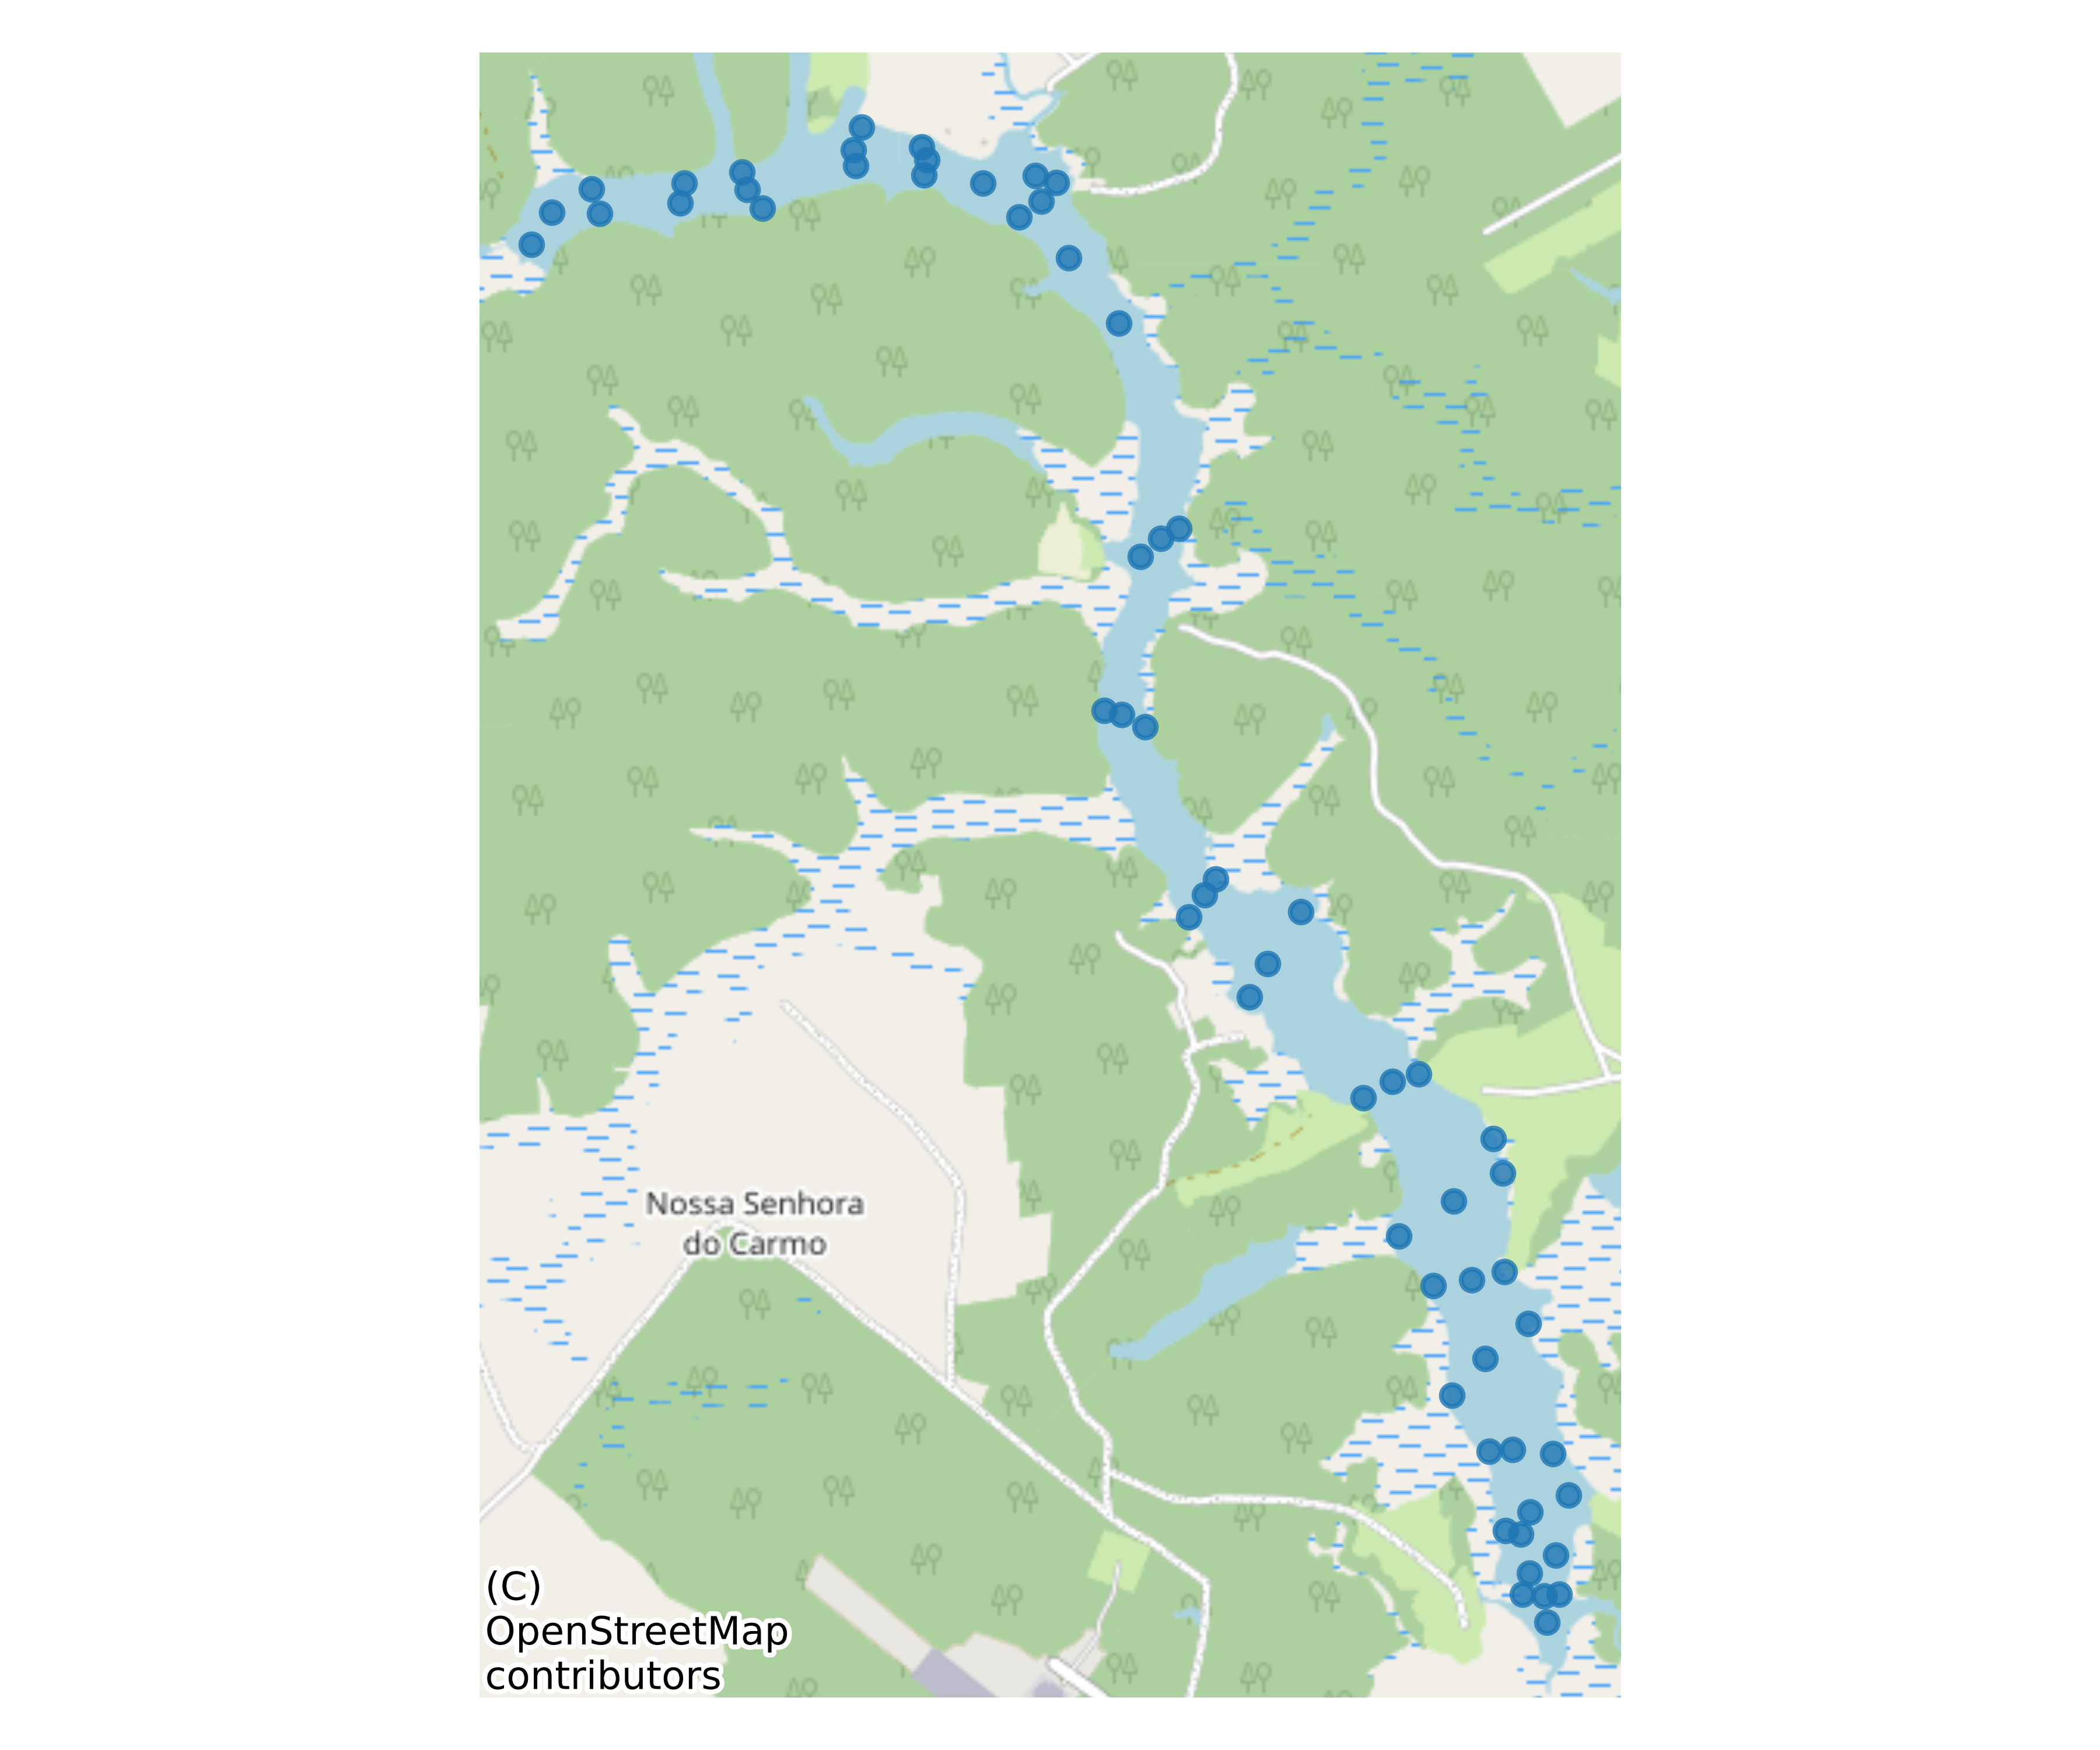
\includegraphics[width=0.78\textwidth]{map_points_osm_21S.png}
\caption{Sampling locations over OpenStreetMap basemap (UTM 21S).}
\label{fig:dataset_map}
\end{figure}

\begin{table}[t]
\caption{Target summary statistics in the original field dataset.}
\label{tab:dataset_stats}
\centering
\begin{tabular}{lcccc}
\toprule
Variable & Mean & Std & Min & Max \\
\midrule
pH & 5.73 & 0.31 & 5.15 & 6.50 \\
OD (mg/L) & 1.86 & 0.32 & 1.26 & 2.52 \\
Turbidity (NTU) & 2.77 & 1.37 & 0.06 & 6.18 \\
\bottomrule
\end{tabular}
\end{table}

\subsection{Data Augmentation}
Because the original dataset is small, synthetic augmentation was applied with factor $\times 10$ using light Gaussian perturbation ($\sigma=0.01$) in normalized space. This strategy was used to stabilize training and reduce split sensitivity, while preserving marginal distributions and physical plausibility. The augmented set is used for training support only and does not represent additional field measurements.

To minimize distortion risk, augmentation was constrained to low-amplitude perturbations and evaluated with distributional checks and ablation analysis. The objective was not to create synthetic dynamics absent from the field campaign, but to increase local density around observed samples and improve optimization stability across randomized splits. In practice, this reduced macro-MAE variability while preserving the same overall value ranges and central tendencies of the original measurements.

Finally, the dataset should be interpreted as an initial regional benchmark rather than a universal hydrological representation. The current sampling supports comparative modeling and deployment analysis, while broader external generalization requires multi-season campaigns and additional freshwater sites with different hydrodynamic and anthropogenic profiles.

\section{Methodology}

\subsection{Multimodal Input Representation}
To avoid ambiguity between symbolic variables and sensor names, we represent each observation using an ordered multimodal feature vector:
\begin{equation}
\mathbf{x} = [x, y, \text{TEMP}, \text{COR}_{A}, \text{COR}_{V}] \in \mathbb{R}^{5},
\end{equation}
and a three-output target vector:
\begin{equation}
\mathbf{y} = [\text{pH}, \text{OD}, \text{TURB}] \in \mathbb{R}^{3}.
\end{equation}
Input features are normalized before spike encoding. We then apply rate coding so that each normalized scalar is converted into a spike train over $T$ time steps, with firing probability proportional to its magnitude. This produces a temporal representation compatible with the downstream LIF dynamics while preserving the multimodal structure of the original sample.

\subsection{SNN Architecture}
The model follows a feed-forward SNN with topology $5 \rightarrow 64 \rightarrow 3$, with a hidden leaky integrate-and-fire (LIF) layer, as illustrated in Fig.~\ref{fig:proposed_arch}. The membrane update is
\begin{equation}
\mathbf{u}_{t+1} = \beta\,\mathbf{u}_{t} + \mathbf{W}\mathbf{s}_{t} - \theta\,\mathbf{z}_{t},
\end{equation}
where $\beta$ is membrane decay, $\theta$ is firing threshold, and $\mathbf{z}_t$ are emitted spikes. Output prediction is computed by temporal aggregation across steps.

\begin{figure}[!htbp]
\centering
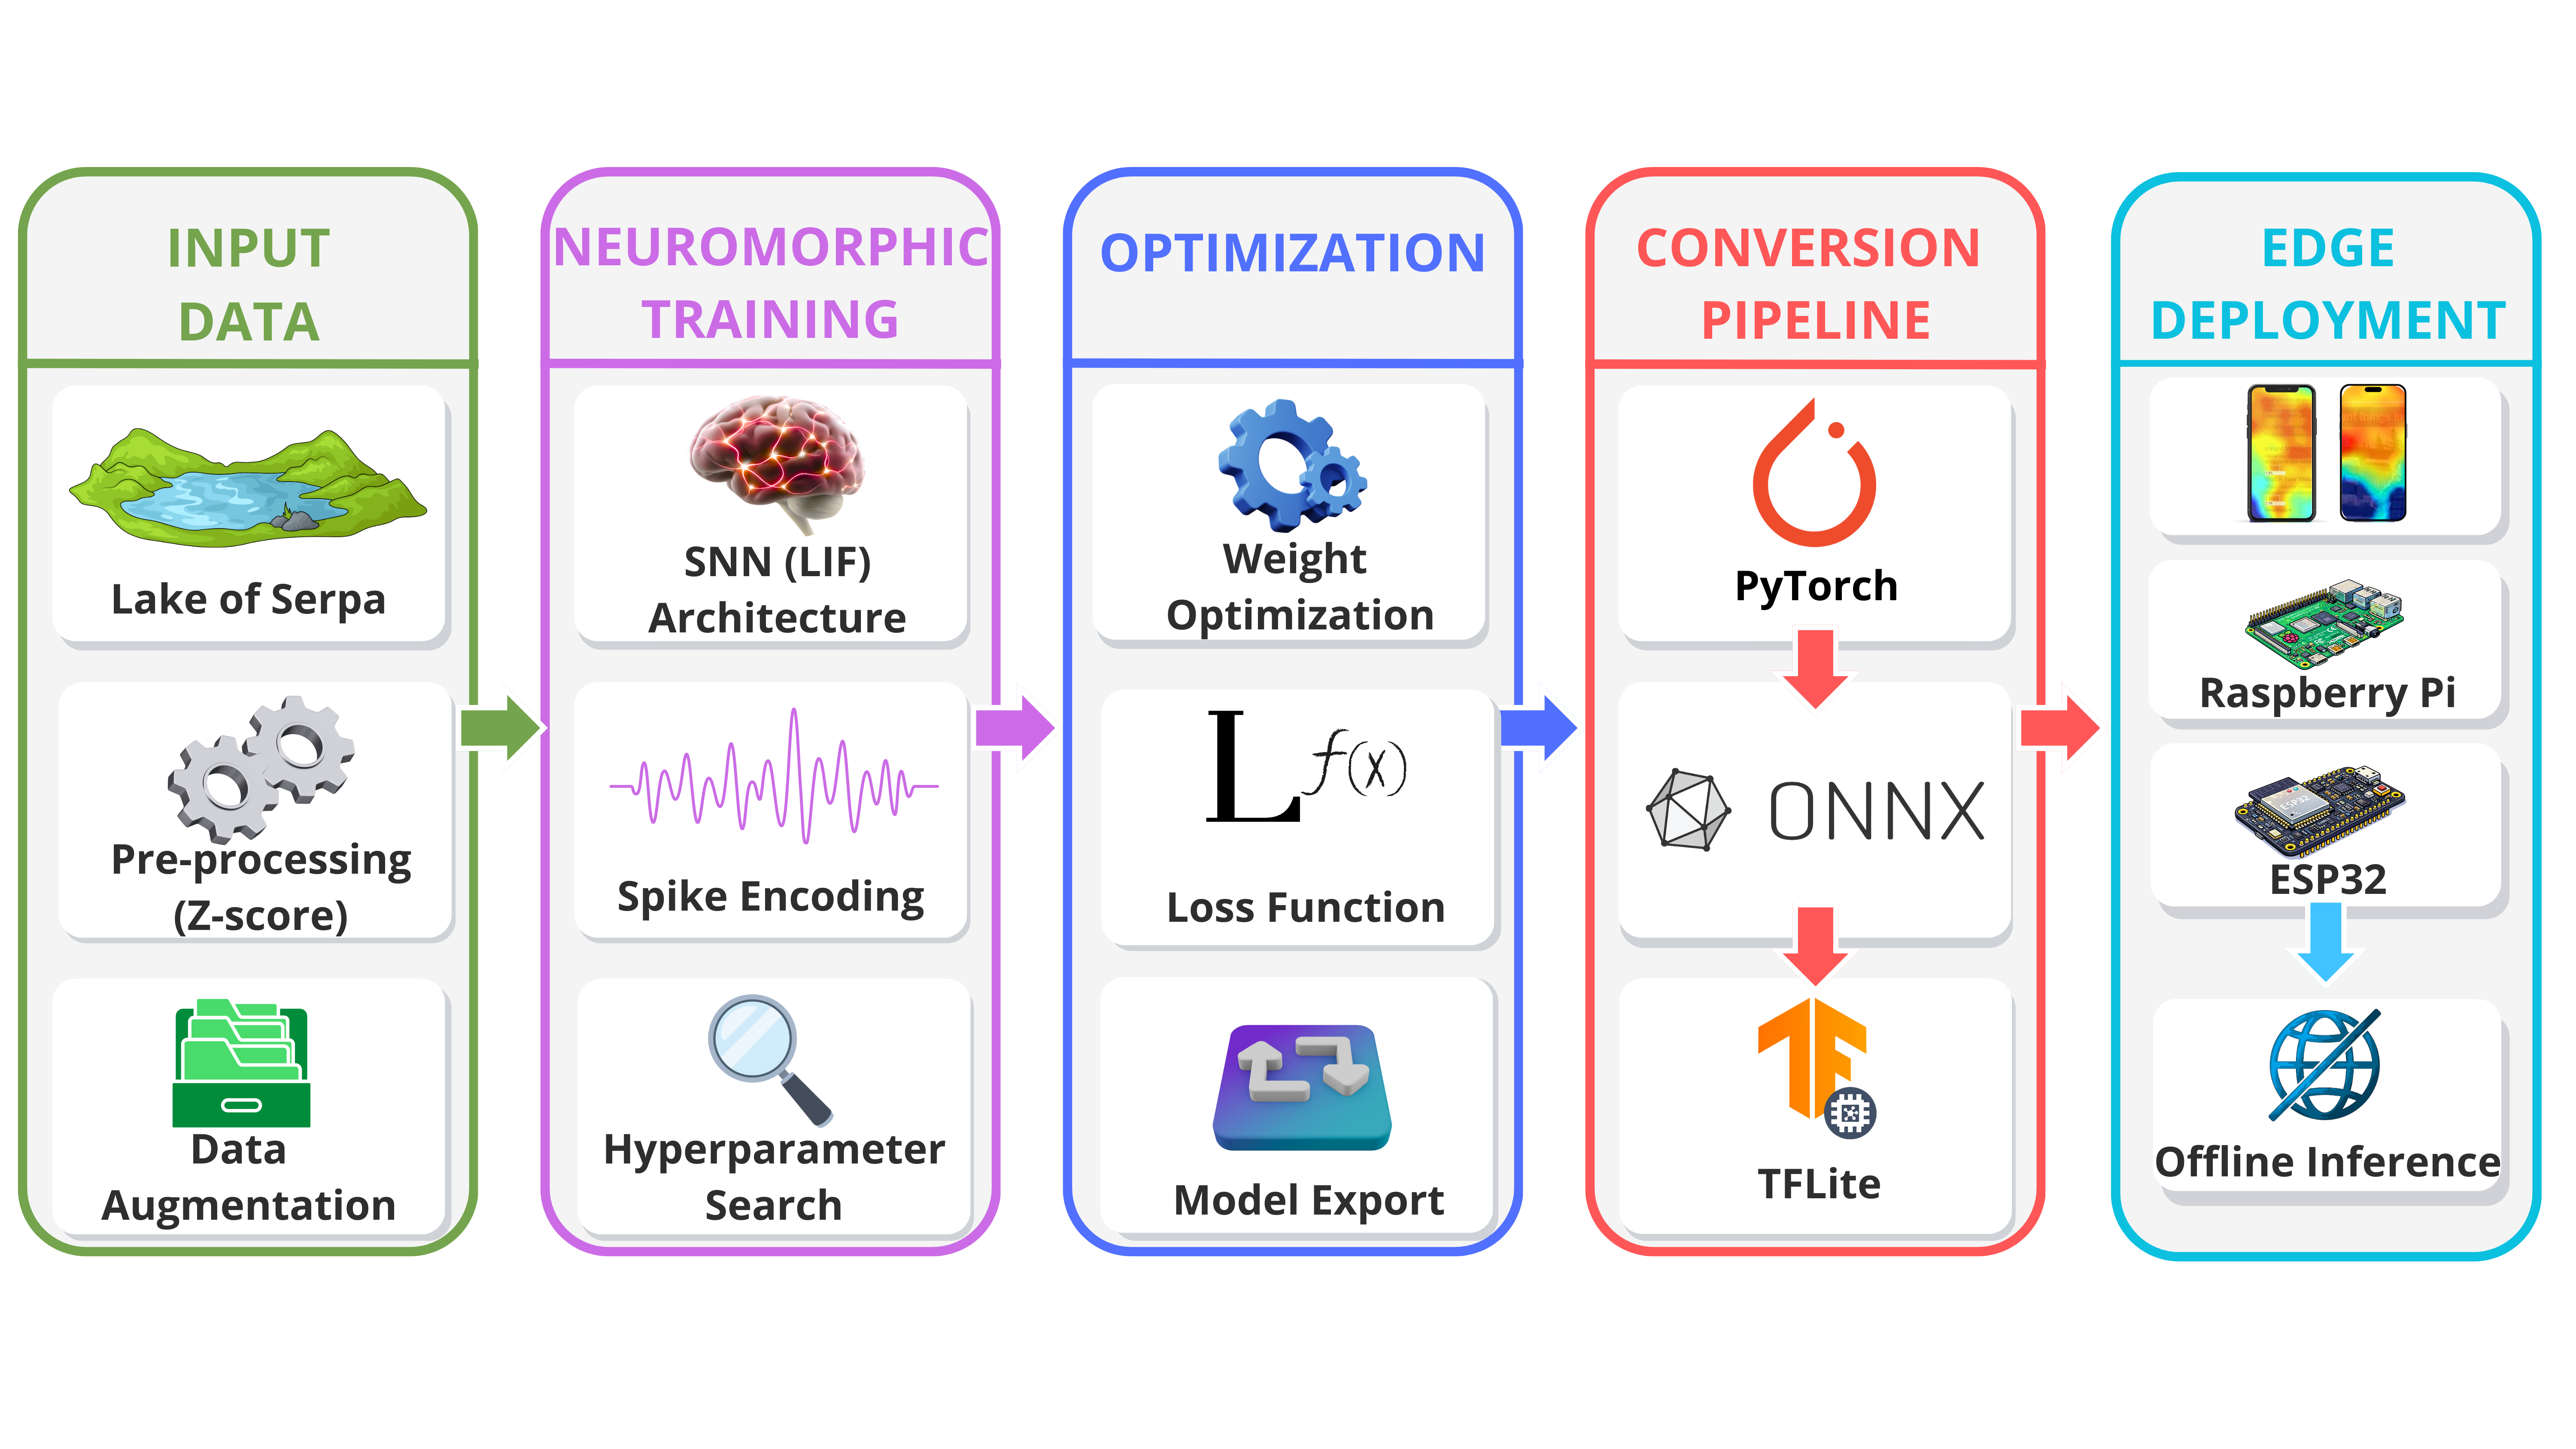
\includegraphics[width=0.86\textwidth]{Arquitetura.png}
\caption{Proposed multimodal SNN architecture for offline edge inference.}
\label{fig:proposed_arch}
\end{figure}

Figure~\ref{fig:proposed_arch} presents the complete end-to-end workflow adopted in this study. The first block consolidates field data preparation, including normalization and controlled augmentation. The second block represents neuromorphic training with LIF neurons, spike encoding, and hyperparameter search. The third block covers model optimization and export of trained parameters. The fourth block defines the interoperability path from PyTorch to ONNX and then to TFLite for lightweight runtime execution. Finally, the fifth block shows edge deployment on heterogeneous platforms (Android, Raspberry Pi, and ESP32), all operating under an offline inference paradigm suitable for low-connectivity monitoring scenarios.

\subsection{Training Protocol}
Training used Adam optimizer and weighted MSE loss with early stopping. Hyperparameters were selected by grid search over hidden size, learning rate, temporal steps $T$, threshold, and decay factor. Evaluation used repeated random seeds and macro metrics (MAE, RMSE, and $R^2$) over the three targets.

As shown in Fig.~\ref{fig:loss_curve_method}, both training and validation losses decrease rapidly in the initial epochs and then converge to a stable plateau with limited divergence. This behavior indicates that the selected configuration reached consistent optimization without strong overfitting patterns, supporting the use of early stopping and confirming that the augmented multimodal training setup improved convergence stability for this small-data regime.

\begin{figure}[!htbp]
\centering
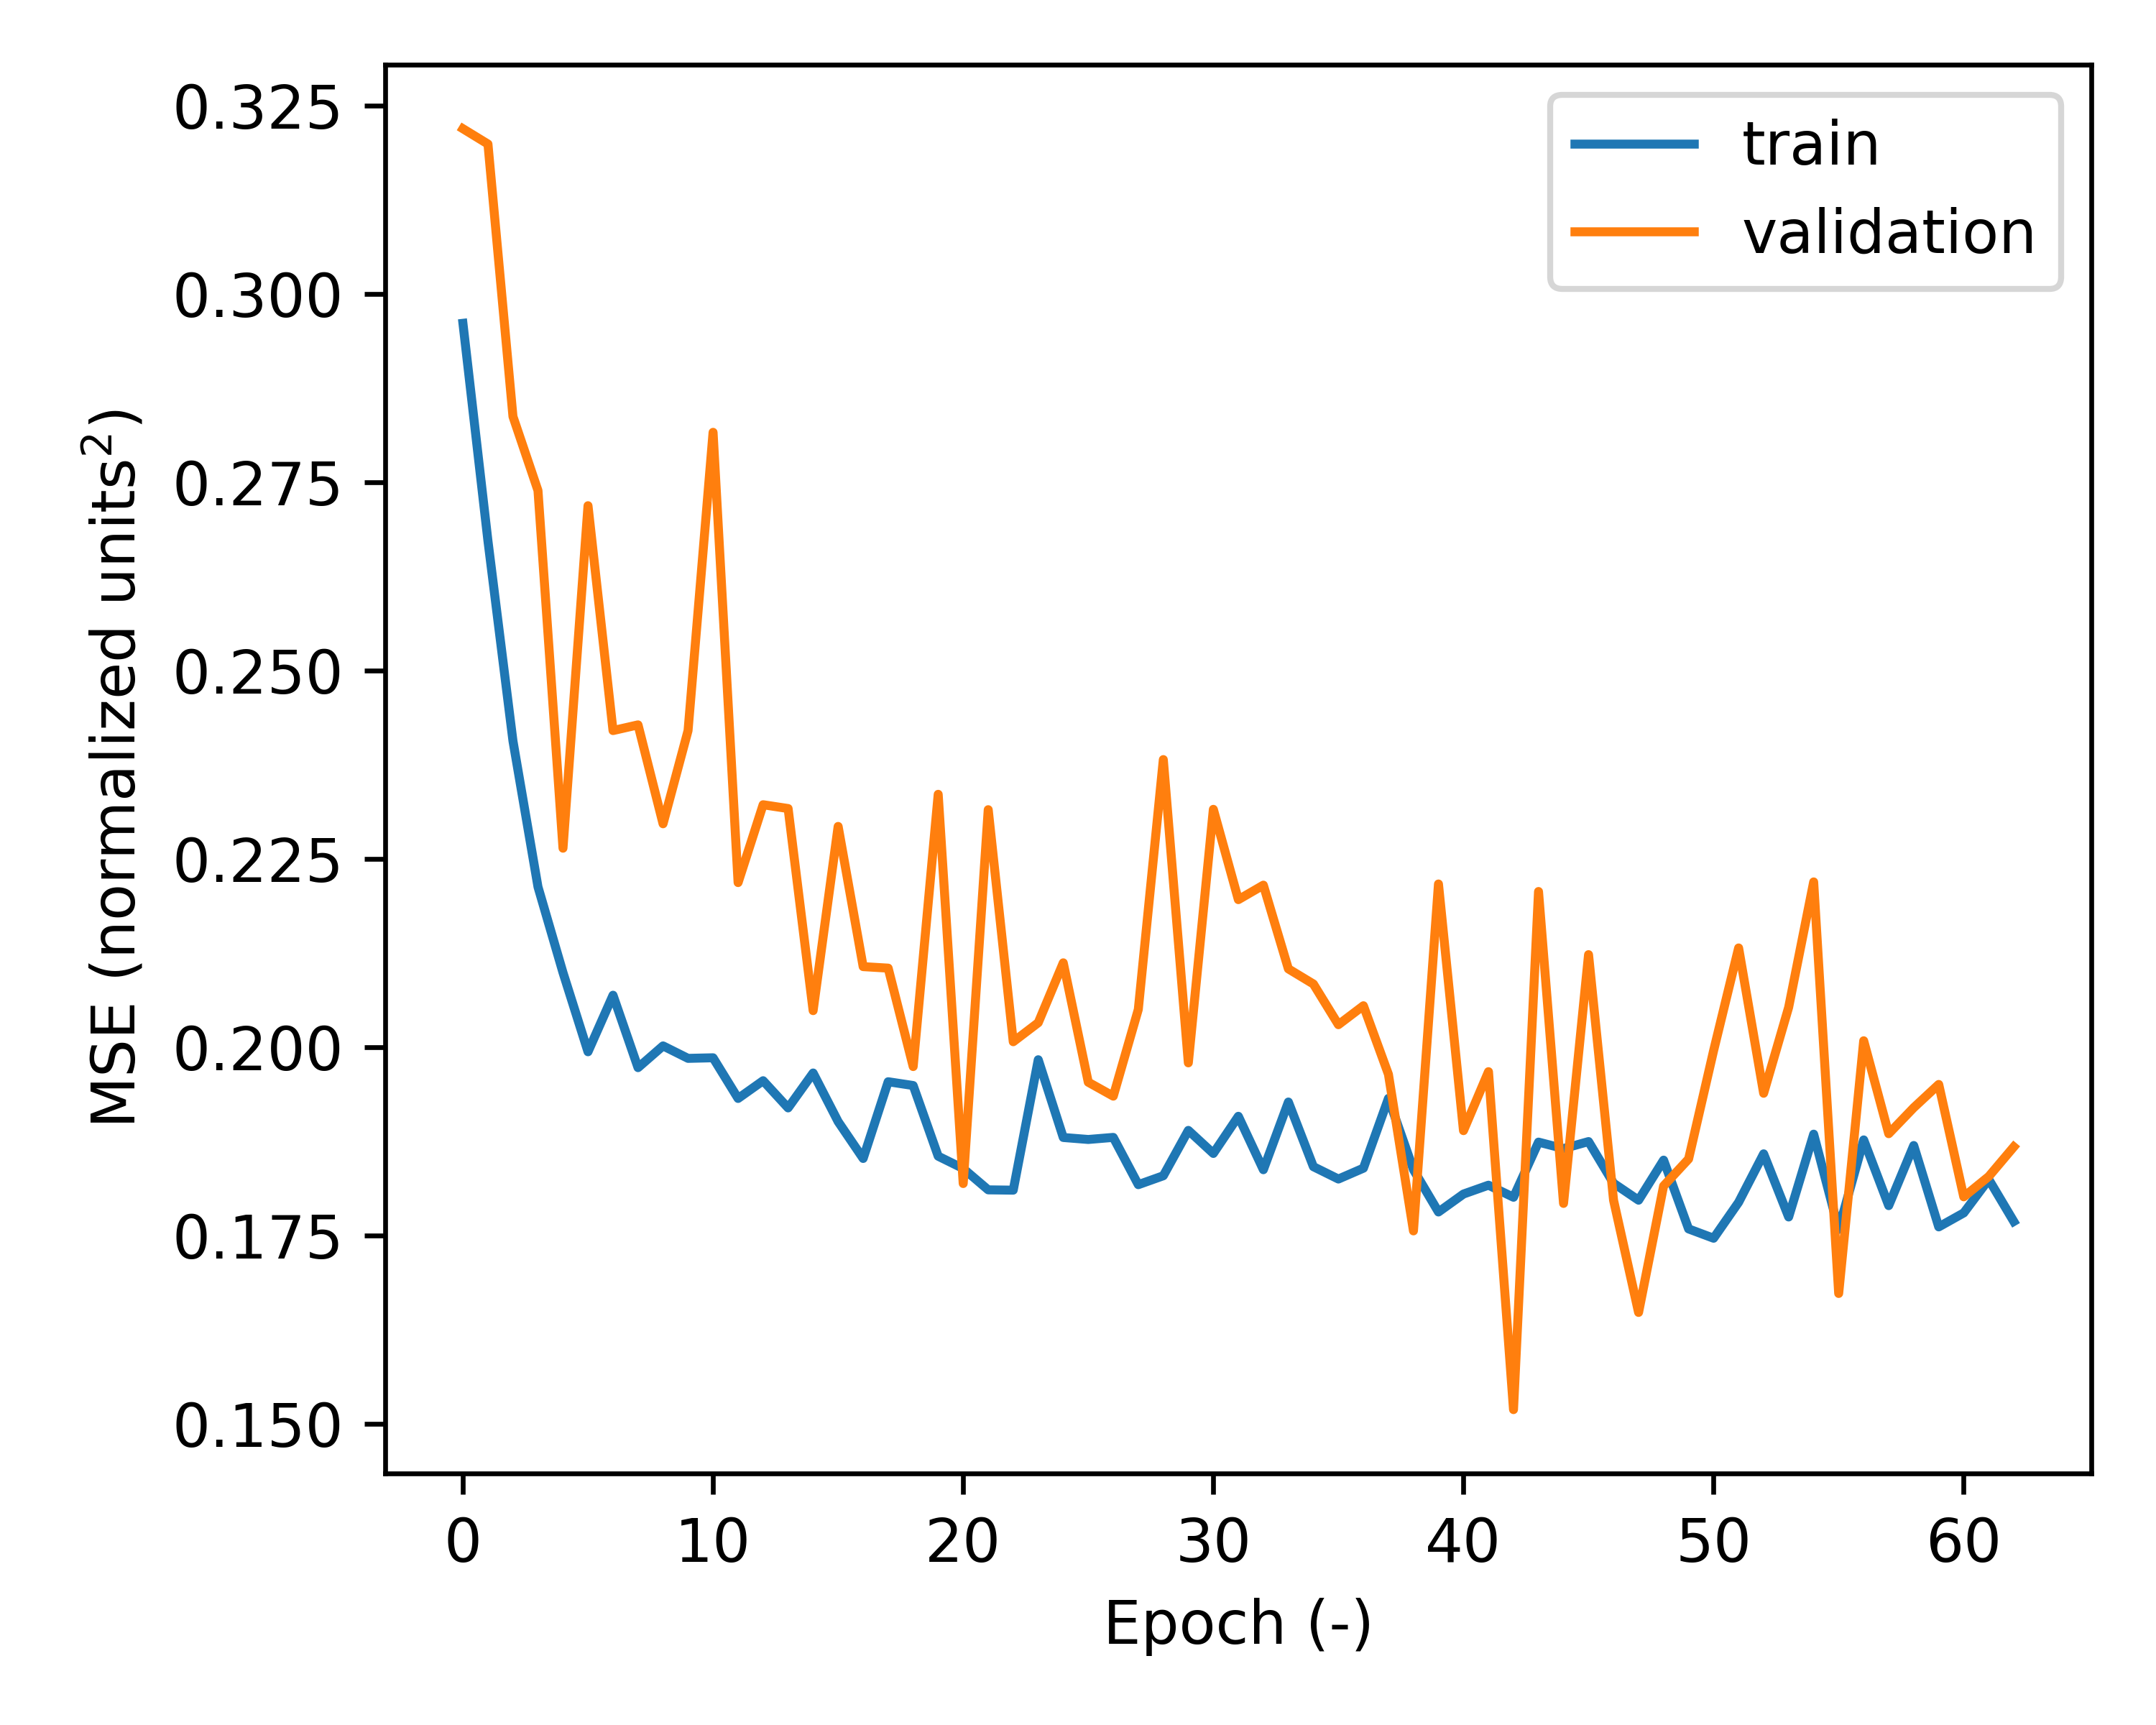
\includegraphics[width=0.5\textwidth]{loss_curve_multi.png}
\caption{Training and validation loss (MSE) of the selected multimodal SNN.}
\label{fig:loss_curve_method}
\end{figure}



\FloatBarrier

\section{Energy Measurement Setup}

\subsection{Instrumentation and Procedure}
\textbf{ESP32 and Raspberry Pi:} current and voltage were sampled every 500 ms using INA219. Two windows were captured: idle ($N_{idle}$ samples) and load ($N_{load}$ samples) during benchmark execution.\newline
\textbf{Android devices:} current and voltage were read from system APIs under controlled idle/load phases.
The complete instrumentation and sampling windows are summarized in Table~\ref{tab:energy_setup}.

Incremental power was estimated as
\begin{equation}
\Delta P = P_{load} - P_{idle},
\end{equation}
and energy per inference as
\begin{equation}
E_{inf} = \frac{\Delta P}{\text{throughput}}.
\end{equation}

\begin{table}[t]
\caption{Measured setup and sampling windows by platform.}
\label{tab:energy_setup}
\centering
\begin{tabular}{lccc}
\toprule
Platform & Sensor/Source & Idle samples & Load samples \\
\midrule
ESP32 (MicroPython) & INA219 & 50 & 50 \\
Raspberry Pi 4B & INA219 & 97 & 440 \\
Android (A/B/C) & System telemetry & 200 & 200 \\
\bottomrule
\end{tabular}
\end{table}


Figure~\ref{fig:speed_energy_setup} summarizes the deployment envelope by combining throughput and incremental energy per inference in a single view. Movement to the right indicates faster processing, while downward movement indicates lower energy cost per prediction. This representation highlights that the best operating point depends on application cadence: high-rate scenarios favor smartphone and SBC execution, whereas low-rate autonomous sensing can still be supported on microcontroller-class hardware.


\begin{figure}[t]
\centering
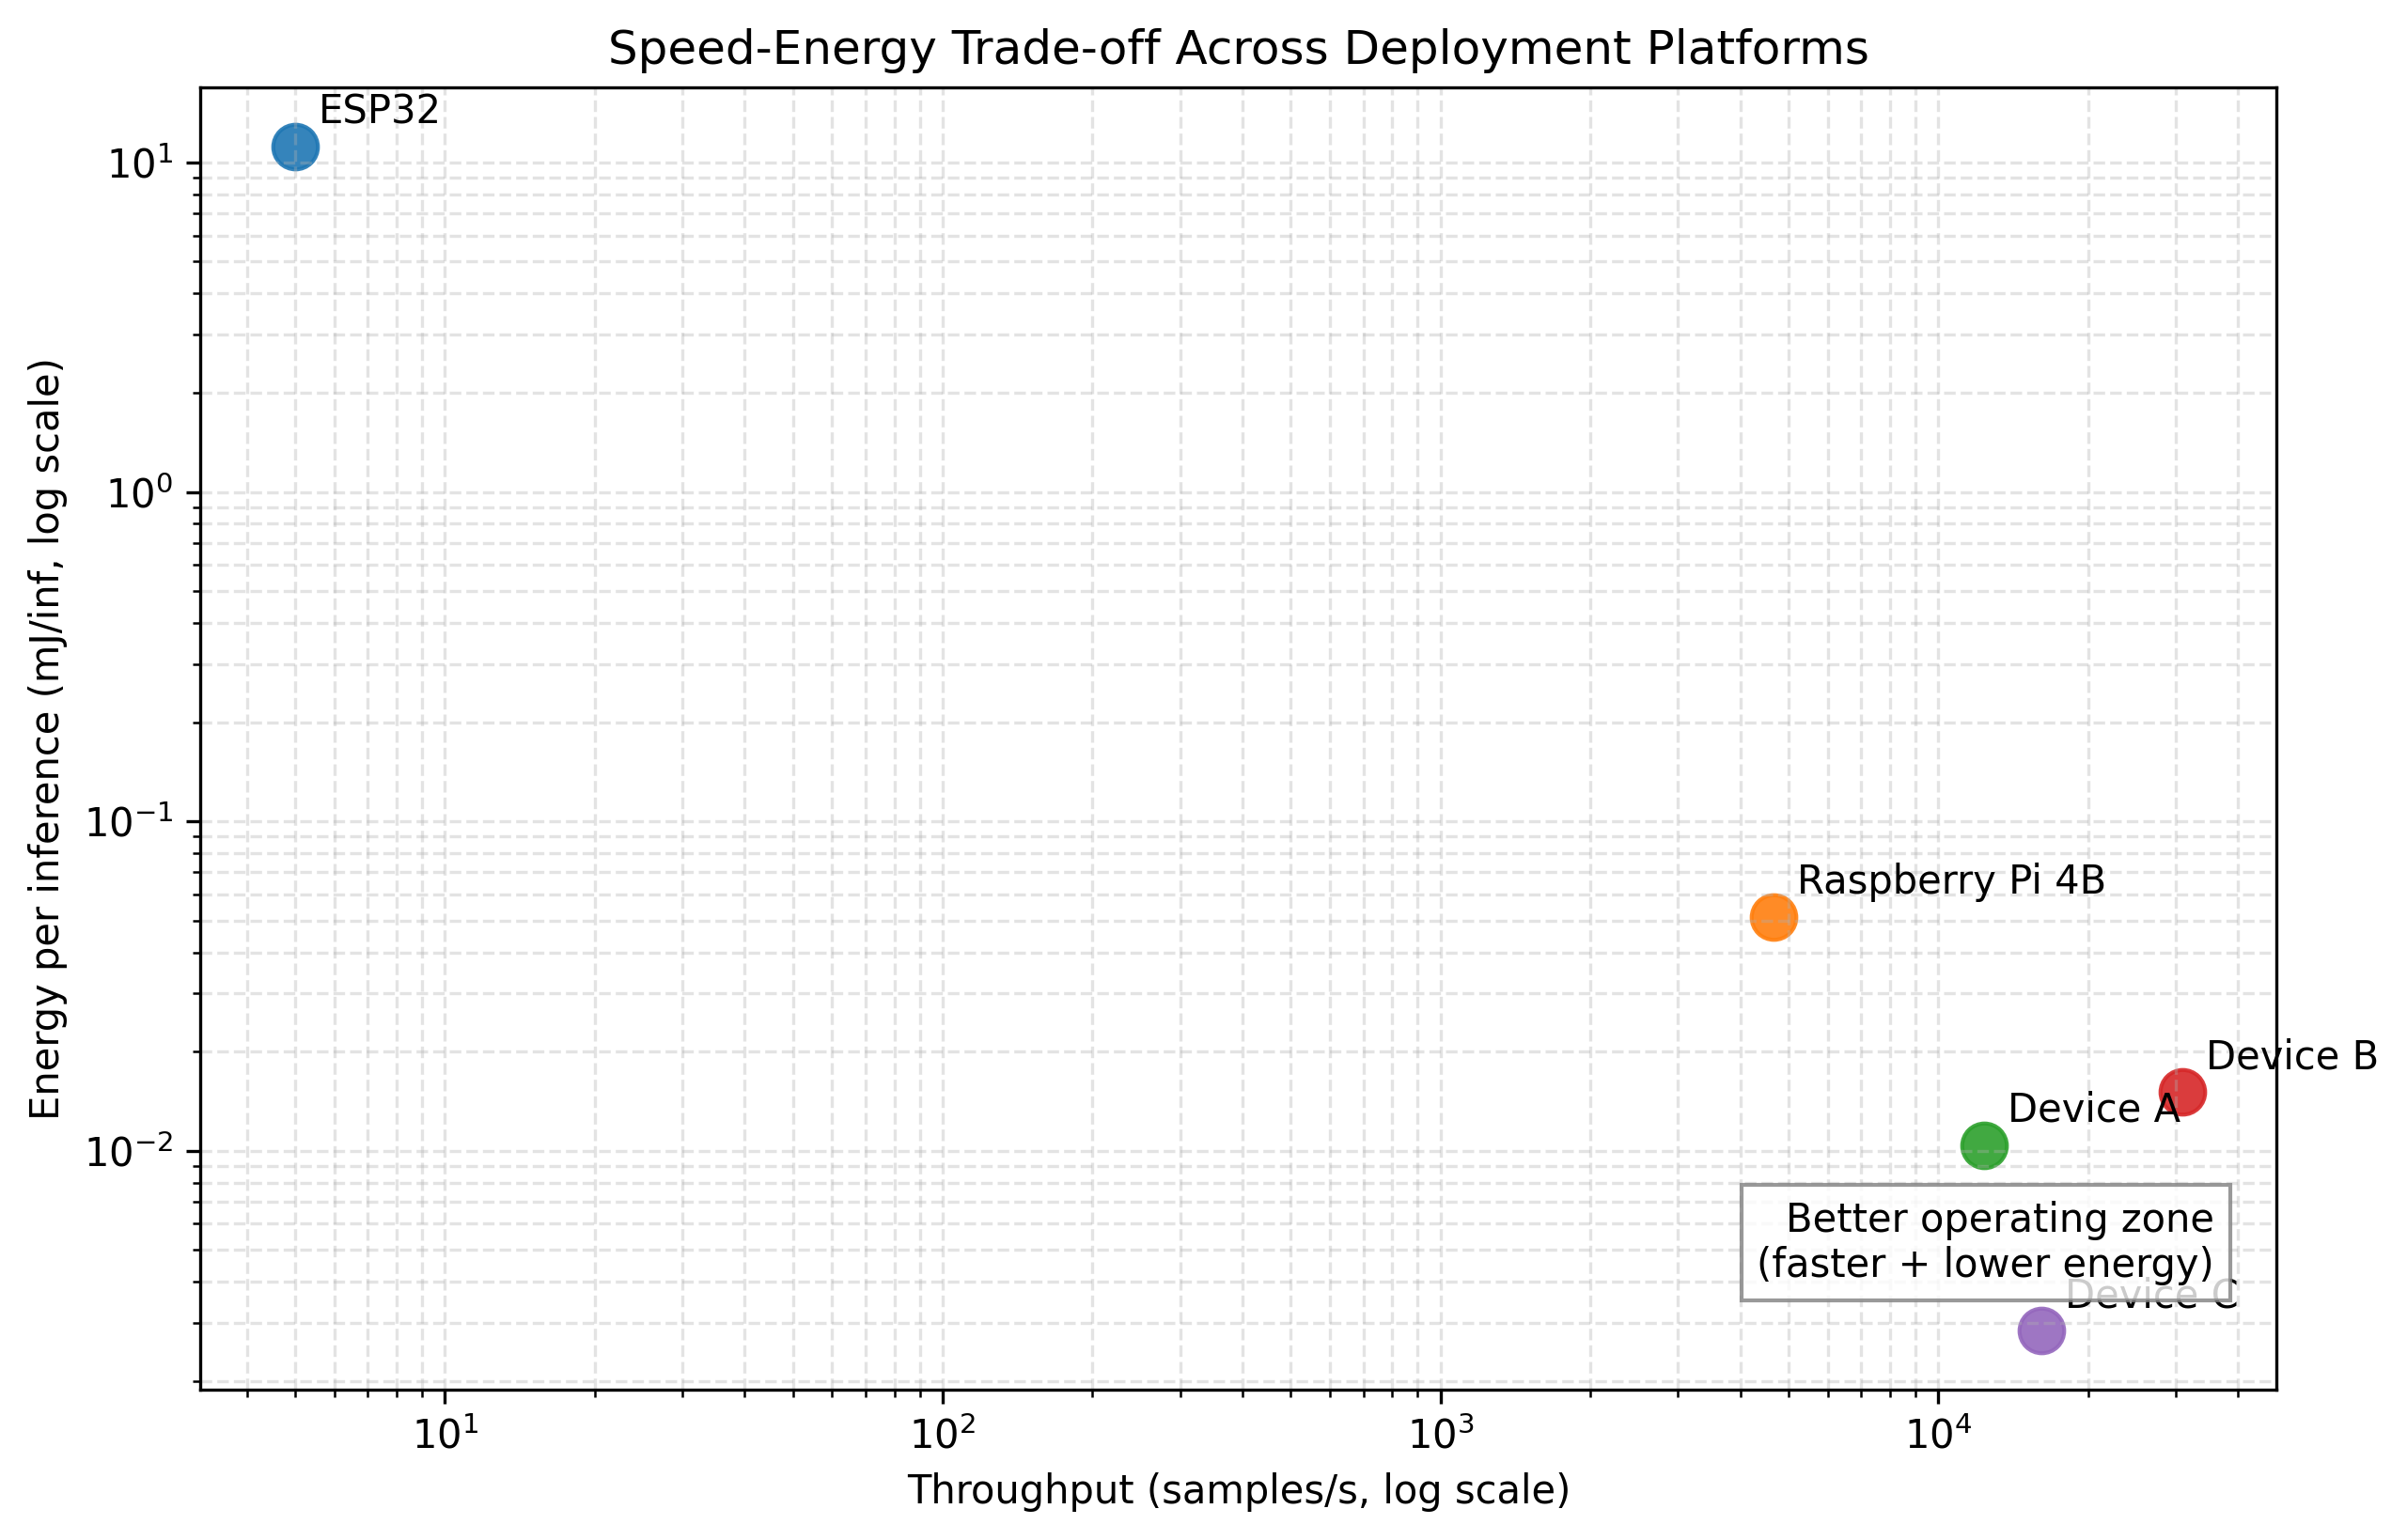
\includegraphics[width=0.88\textwidth]{speed_energy_tradeoff.png}
\caption{Speed--energy positioning of evaluated platforms (log scales).}
\label{fig:speed_energy_setup}
\end{figure}

\section{Experimental Results}

\subsection{Prediction Performance}
Table~\ref{tab:pred_perf} summarizes macro performance across compared models in the multimodal task. Random Forest achieved the lowest average error, while the SNN remained competitive and more stable than a simple MLP baseline.

\begin{table}[!h]
\caption{Multimodal prediction performance (macro metrics).}
\label{tab:pred_perf}
\centering
\begin{tabular}{lccc}
\toprule
Model & MAE & RMSE & $R^2$ \\
\midrule
Random Forest & 0.438 & 0.572 & 0.350 \\
LSTM & 0.455 & 0.593 & 0.322 \\
SNN (proposed) & 0.483 & 0.617 & 0.256 \\
MLP & 0.560 & 0.694 & 0.180 \\
\bottomrule
\end{tabular}
\end{table}

The numerical ranking indicates that Random Forest achieves the lowest MAE, while the proposed SNN remains in a competitive range and preserves the edge-oriented advantages discussed in this paper, especially when considering deployment constraints beyond pure predictive accuracy.

\subsection{Energy Consumption and Latency}
Table~\ref{tab:energy_latency} reports incremental energy-per-inference and throughput across deployment platforms. ESP32 is feasible for low-rate autonomous scenarios but has higher energy per inference due to limited throughput. Raspberry Pi and Android devices provide much lower mJ/inf in high-throughput settings.

\begin{table}[!htbp]
\caption{Latency/throughput and incremental energy across platforms.}
\label{tab:energy_latency}
\centering
\begin{tabular}{lccc}
\toprule
Platform & Throughput (samples/s) & $\Delta P$ (W) & Energy (mJ/inf) \\
\midrule
ESP32 (MicroPython) & 5.0 & 0.056 & 11.204 \\
Raspberry Pi 4B & 4670.50 & 0.239 & 0.0512 \\
Device A (Android) & 12337.40 & 0.128 & 0.0104 \\
Device B (Android) & 30905.08 & 0.468 & 0.0151 \\
Device C (Android) & 16121.71 & 0.046 & 0.00285 \\
\bottomrule
\end{tabular}
\end{table}

Figure~\ref{fig:energy_bar_lnncs} compares the incremental energy per inference across deployment platforms using a logarithmic scale to preserve visual readability despite large magnitude differences. The plot shows that ESP32 has the highest energy cost per prediction, mainly due to its low throughput, while Raspberry Pi and Android devices operate in a much lower mJ/inf range. Among mobile platforms, the figure also highlights that higher throughput does not always imply lower energy per inference, reinforcing that platform selection should be based on the joint analysis of processing speed and incremental power behavior under real deployment conditions.

\begin{figure}[!htbp]
\centering
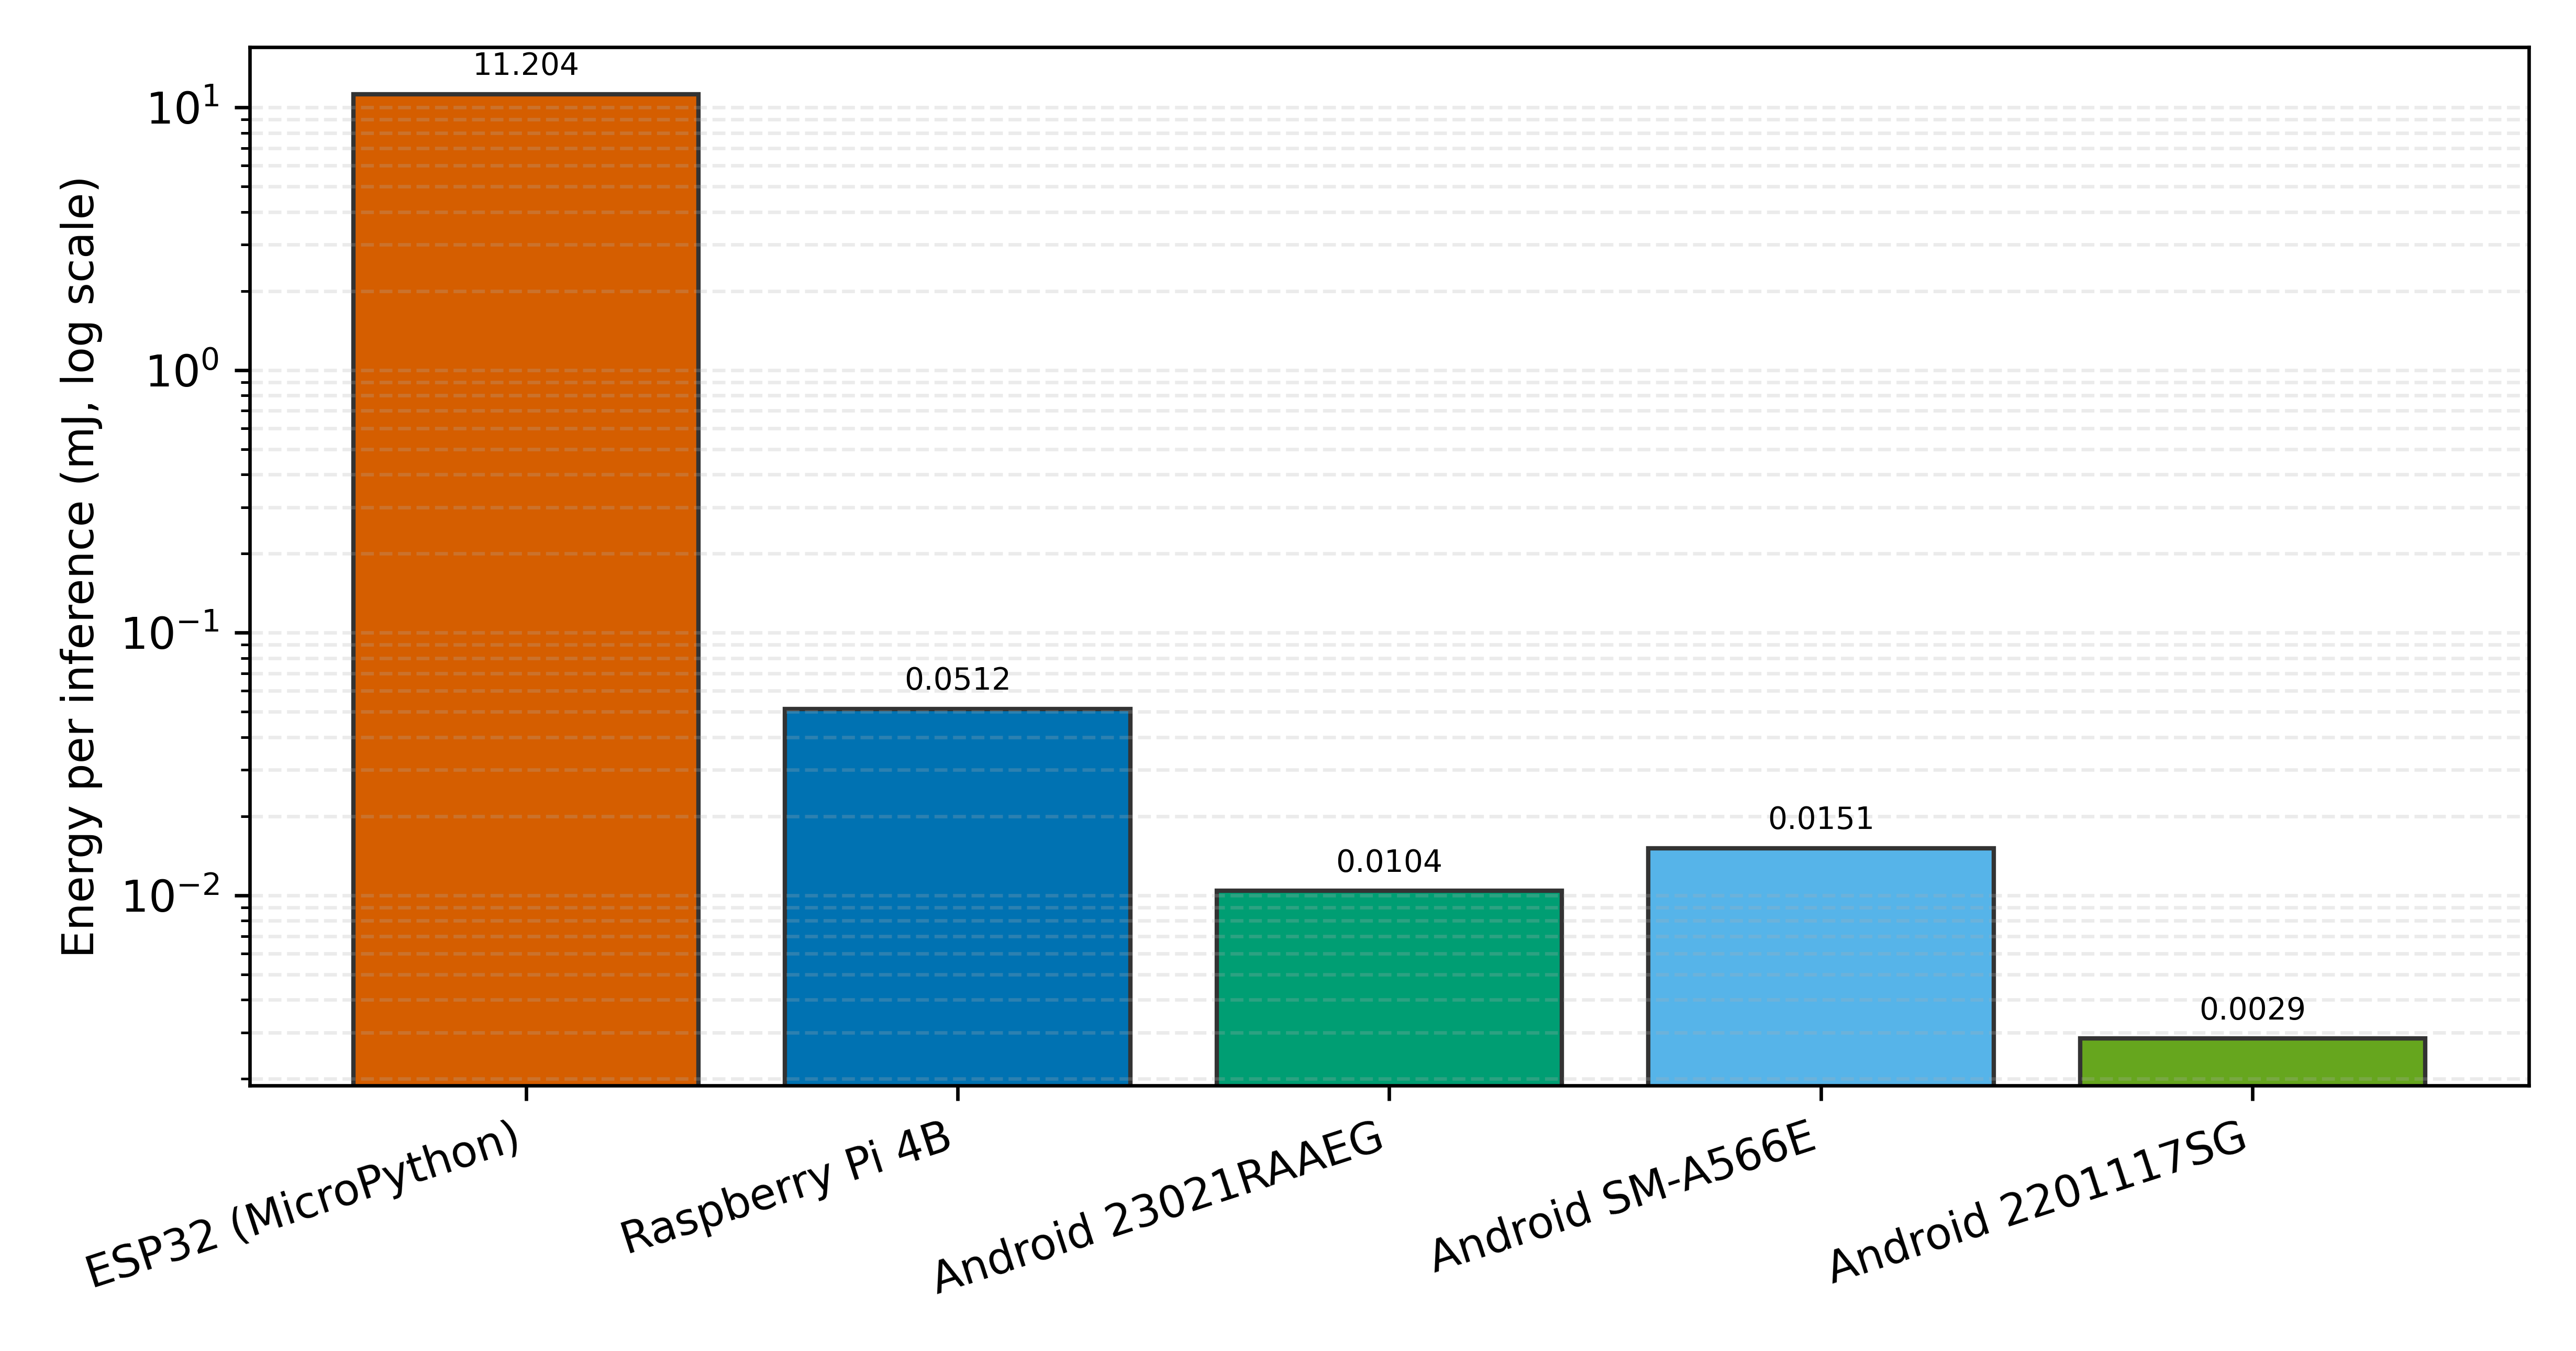
\includegraphics[width=0.82\textwidth]{energy_platforms_bar.png}
\caption{Comparative energy per inference (log scale).}
\label{fig:energy_bar_lnncs}
\end{figure}

Figure~\ref{fig:energy_bar_lnncs} complements Table~\ref{tab:energy_latency} by making the large energy gap between ESP32 and higher-throughput platforms visually explicit on a logarithmic axis. Without log scaling, low-mJ/inf differences among Raspberry Pi and Android devices would be visually compressed; with this scale, relative efficiency differences remain readable and directly comparable.

\FloatBarrier

\section{Discussion}

Results show a clear trade-off between predictive accuracy and deployment constraints. Although Random Forest reached slightly lower MAE, the SNN remained competitive while offering event-driven temporal processing and direct alignment with neuromorphic edge deployment goals. This is relevant for low-power autonomous monitoring where model choice is not driven by accuracy alone. From a methodological standpoint, the multimodal setup proved valuable because it keeps physically related targets in a single inference pipeline and simplifies downstream decision logic in field applications. The observed error profile also indicates nonuniform target difficulty: pH and OD were more stable, while turbidity concentrated a larger share of uncertainty. This asymmetry is expected in heterogeneous freshwater environments and supports the use of weighted losses, repeated-seed reporting, and per-target diagnostics rather than relying on a single aggregate metric.

From the systems perspective, platform behavior is heterogeneous: Device B reached the highest throughput, Device C achieved the lowest incremental energy per inference, and ESP32 provided full offline feasibility at much lower processing rates. Therefore, deployment decisions should be scenario-dependent: high-rate analytics benefit from smartphone/SBC-class hardware, while sparse periodic sensing can still be addressed by microcontrollers. Energy interpretation should be made with explicit operational context, since baseline platform power varies with architecture and operating-system behavior. For this reason, energy per inference combined with throughput is a more actionable criterion than absolute watts alone. The environmental interpretation is consistent with the literature and regulatory practice, but generalization remains limited by dataset size. Augmentation and multi-seed evaluation reduced split sensitivity, yet broader field campaigns are still required for stronger external validity. Offline inference remains a practical advantage in low-connectivity regions by preserving local prediction and screening without cloud dependence.

\section{Conclusion}

This paper presented an energy-aware offline multimodal SNN pipeline for water-quality prediction in an Amazonian edge-monitoring context. The proposed approach demonstrated practical feasibility from training to deployment, including geospatial interpretation and cross-platform latency/energy benchmarking. The results indicate that neuromorphic inference is deployable under real hardware constraints, with measurable platform-specific trade-offs between throughput and energy per inference. While not always the best in absolute MAE, the SNN remains a robust option when temporal event-driven processing and edge compatibility are first-class requirements.

Threats to validity should be explicitly considered when interpreting these findings. The main internal-validity risk is the limited size of the original field dataset, which can increase split sensitivity and make small metric gaps unstable across partitions; this was mitigated through repeated-seed evaluation, conservative augmentation, and per-target reporting, but not fully eliminated. External validity is also bounded by hydrological diversity across Amazonian subregions, so broader regional claims require multi-site, multi-season campaigns with harmonized acquisition protocols. Future work includes broader field acquisition across seasonal regimes, external validation in additional freshwater systems, and deeper co-optimization of encoding parameters and hardware execution modes for improved energy-performance balance.

\section*{Acknowledgments}

The authors thank the Automation, Computer Vision, Artificial Intelligence, and Robotics Laboratory (NAVIR), the Graduate Program in Science, Technology and Health (PPGCTS), and the Federal University of Amazonas (UFAM). The authors also acknowledge the Eldorado Research Institute, CNPJ 02.437.460/0005-30, Manaus, Amazonas, Brazil, particularly its Manaus Operations Department (DOM). Furthermore, the authors acknowledge Motorola Mobility Comércio de Produtos Eletrônicos Ltda and Flextronics da Amazônia Ltda, as provided for in Articles 21 and 22 of Decree No. 10.521/2020, under Federal Law No. 8.387/1991 and Agreement No. 008/2024, signed with ICET/UFAM, through the Research, Development, and Technological Innovation Project (PDI) “Mob4Ai – Advanced Artificial Intelligence for Neuromorphic Mobile Systems.”


\bibliographystyle{splncs04}
\bibliography{references}

\end{document}
